\documentclass[main.tex,fontsize=8pt,paper=a4,paper=portrait,DIV=calc,]{scrartcl}
% Document
\usepackage[T1]{fontenc}
\usepackage[utf8]{inputenc}
\usepackage[dvipsnames]{xcolor}
\usepackage[nswissgerman,english]{babel} 
\usepackage{hyperref}
\renewcommand{\familydefault}{\sfdefault}

% Format
\usepackage[top=5mm,bottom=1mm,left=5mm,right=5mm]{geometry}
%\setlength{\headheight}{\baselineskip}
%\setlength{\headsep}{0mm}

%\usepackage{scrlayer-scrpage}
%\clearpairofpagestyles
%\chead{{\bfseries\TITLE, \AUTHOR, \pagename~\thepage}}

%\addtokomafont{pagehead}{\upshape}

\usepackage{multicol}
\setlength{\columnsep}{2mm}
\setlength{\columnseprule}{0.1pt}

% Math
\usepackage{amsmath}
\usepackage{amssymb}
\usepackage{amsfonts}

% Code
\usepackage{fancyvrb, etoolbox, listings, xcolor}
%\usemintedstyle{bw}

%\newminted[shell]{bash}{
%fontsize=\footnotesize,
%fontfamily=tt,
%breaklines=true,
%frame=single,
%framerule=0.1pt,
%framesep=2mm,
%tabsize=2
%}
%\newminted{css}{
%breaklines=true,
%tabsize=4,
%autogobble=true,
%escapeinside=||,
%stripall=true,
%stripnl=true,
%}

    \definecolor{lightgray}{rgb}{0.95, 0.95, 0.95}
    \definecolor{darkgray}{rgb}{0.4, 0.4, 0.4}
    \definecolor{purple}{rgb}{0.65, 0.12, 0.82}
    \definecolor{ocherCode}{rgb}{1, 0.5, 0} % #FF7F00 -> rgb(239, 169, 0)
    \definecolor{blueCode}{rgb}{0, 0, 0.93} % #0000EE -> rgb(0, 0, 238)
    \definecolor{greenCode}{rgb}{0, 0.6, 0} % #009900 -> rgb(0, 153, 0)
    \definecolor{teal}{rgb}{0.0, 0.5, 0.5}

\lstdefinestyle{code}{
    identifierstyle=\color{black},
    keywordstyle=\color{blue}\bfseries\small,
    ndkeywordstyle=\color{greenCode}\bfseries\small,
    stringstyle=\color{ocherCode}\ttfamily\small,
    commentstyle=\color{teal}\ttfamily\textit\small,
    basicstyle=\ttfamily\small,
    breakatwhitespace=false,         
    breaklines=true,                 
    captionpos=b,                    
    keepspaces=true,                 
    showspaces=false,                
    showstringspaces=false,
    showtabs=false,                  
    tabsize=2,
    belowskip=-5pt
}



% Images
\usepackage{graphicx}
\newcommand{\pic}{\includegraphics[scale=0.3]}
\graphicspath{{Screenshots/}{../Screenshots}}
\makeatletter
\def\pictext#1#2{%
    \@ifnextchar[{%
    \pictext@iiiii{#1}{#2}%
    }{%
      \pictext@iiiii{#1}{#2}[0.5,0.4,0.3]% Default is 5
    }%
}
\def\pictext@iiiii#1#2[#3,#4,#5]{\begin{minipage}{#3\textwidth}\includegraphics[scale=#4]{#1}\end{minipage}\begin{minipage}{#5\textwidth}#2\end{minipage}}
\def\minipg#1#2{%
    \@ifnextchar[{%
    \minipg@iiii{#1}{#2}%
    }{%
      \minipg@iiii{#1}{#2}[0.3,0.6]% Default is 5
    }%
}
\def\minipg@iiii#1#2[#3,#4]{\vspace{0.8mm}\begin{minipage}{#3\textwidth}#1\end{minipage}\begin{minipage}{#4\textwidth}#2\end{minipage}{\vspace{0.8mm}}}
\makeatother

%\newenvironment{minty}[2]% environment name
%{% begin code
%  \begin{minipage}{#1}
%  \begin{minted}{#2}
%}%
%{% end code
%  \end{minted}
%  \end{minipage}
%  \end{minty}\ignorespacesafterend
%} 

% Smaller Lists
\usepackage{enumitem}
\setlist[itemize,enumerate]{leftmargin=3mm, labelindent=0mm, labelwidth=1mm, labelsep=1mm, nosep}
\setlist[description]{leftmargin=0mm, nosep}
\setlength{\parindent}{0cm}

% Smaller Titles
\usepackage[explicit]{titlesec}

%% Color Boxes
\newcommand{\sectioncolor}[1]{\colorbox{black!60}{\parbox{0.989\linewidth}{\color{white}#1}}}
\newcommand{\subsectioncolor}[1]{\colorbox{black!50}{\parbox{0.989\linewidth}{\color{white}#1}}}
\newcommand{\subsubsectioncolor}[1]{\colorbox{black!40}{\parbox{0.989\linewidth}{\color{white}#1}}}
\newcommand{\paragraphcolor}[1]{\colorbox{black!30}{\parbox{0.989\linewidth}{\color{white}#1}}}
\newcommand{\subparagraphcolor}[1]{\colorbox{black!20}{\parbox{0.989\linewidth}{\color{white}#1}}}

%% Title Format
\titleformat{\section}{\vspace{0.5mm}\bfseries}{}{0mm}{\sectioncolor{\thesection~#1}}[{\vspace{0.5mm}}]
\titleformat{\subsection}{\vspace{0.5mm}\bfseries}{}{0mm}{\subsectioncolor{\thesubsection~#1}}[{\vspace{0.5mm}}]
\titleformat{\subsubsection}{\vspace{0.5mm}\bfseries}{}{0mm}{\subsubsectioncolor{\thesubsubsection~#1}}[{\vspace{0.5mm}}]
\titleformat{\paragraph}{\vspace{0.5mm}\bfseries}{}{0mm}{\paragraphcolor{\theparagraph~#1}}[{\vspace{0.5mm}}]
\titleformat{\subparagraph}{\vspace{0.5mm}\bfseries}{}{0mm}{\subparagraphcolor{\thesubparagraph~#1}}[{\vspace{0.5mm}}]

%% Title Spacing
\titlespacing{\section}{0mm}{0mm}{0mm}
\titlespacing{\subsection}{0mm}{0mm}{0mm}
\titlespacing{\subsubsection}{0mm}{0mm}{0mm}
\titlespacing{\paragraph}{0mm}{0mm}{0mm}
\titlespacing{\subparagraph}{0mm}{0mm}{0mm}

%% format cells
\usepackage[document]{ragged2e}
\usepackage{array, makecell}
\renewcommand{\arraystretch}{2}
\newcommand{\mc}{\makecell[{{m{1\linewidth}}}]}



\begin{document}
\tableofcontents

\lstset{
    language=c++,
    style=code,
}

\newcommand{\TITLE}{CPP Advanced}
\newcommand{\AUTHOR}{Fabio Lenherr}
\setcounter{tocdepth}{1}

\section{Move Semantics}

\subsection{Copy}
\textcolor{purple}{By default cpp will always create copies, this is good for memory safety etc, as you will not be returning null values, but it can be a runtime hit!}\newline
\textcolor{teal}{(There are some special types that can't be copied like mutexes etc)}
\begin{lstlisting}
// Copy contructor
class something {
  something(const something &other) {
    // copy values from other
  }
}
\end{lstlisting}

\subsection{Move}
\textcolor{purple}{Move constructor will \emph{NOT copy values, instead, it will move these values into the new object, this is better for performance, but it requires more management from the programmer!}}\newline
\textcolor{teal}{Make sure to free the memory at the old object, otherwise you might be dealing with nullpointers!}
\begin{lstlisting}
Vector(Vector<T> &&vec)
    : size(vec.size), cap(vec.cap), data(std::move(vec.data)) {
  vec.data = nullptr;
} // yes this is the vector that you implemented kekw
\end{lstlisting}
\textcolor{red}{In short, the move constructor makes a lot of sense when you have \emph{Heap data}, aka if you have something like an array or a vector, then you will want to make sure to always use the move constructor if you can do so.}\newline
The default move constructor is as follows:
\begin{lstlisting}
struct S {
  S(S && s) : member{std::move(s.member)}
  {...}
  M member;
};
\end{lstlisting}

\subsection{Copy Assignment}
Default copy assignment constructor:
\begin{lstlisting}
struct S {
  auto operator=(S const& s) -> S& {
     member = s.member;
     return *this;
  }
  M member;
};
\end{lstlisting}

\subsection{Move Assignment}
Default move assignment constructor:
\begin{lstlisting}
struct S {
  auto operator=(S&& s) -> S& {
    member = std::move(s.member);
    return *this;
  }
  M member;
};
\end{lstlisting}

\subsection{Rvalue and Lvalue}
\textcolor{purple}{lvalue T\&: \emph{variable with some location in ram}, either on the stack or on the heap.}\newline
\textcolor{purple}{rvalue T\&\&: \emph{temporary value} that has no variable and no location in memory, it only exists in code.}\newline
\begin{lstlisting}
int a = 5;
// 5 is an r value, it has no memory location
// a is an lvalue -> some address is set to 5

int b = 10;

int c = a + b;
// a + b is an rvalue -> value is 15, but no memory location for this calculation
// c is an lvalue -> some address is set to 5
\end{lstlisting}

\subsubsection{Convert lvalue to rvalue}
\textcolor{purple}{By default you can't just use an lvalue as an rvalue, however, you can use \emph{std::move} to explicitly convert an lvalue to an rvalue.\newline
Note that in this case, you \emph{can't use the old variable anymore, as the data has been moved! -> see rust}}
\begin{lstlisting}
auto consume(Food&& food) -> void;

auto fryBurger() -> Food;
auto fastFood() -> void {
  Food fries{"salty and greasy"};
  consume(fryBurger()); //call with rvalue
  consume(fries); //cannot pass lvalue to rvalue reference
  consume(std::move(fries)); //explicit conversion lvalue to xvalue
  Food&& burger = fryBurger(); //life-extension of temporary
}
\end{lstlisting}

\subsection{Other value types}
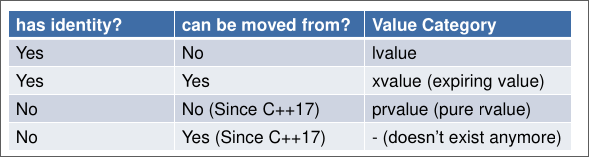
\includegraphics[scale=0.4]{2023_02_28_01_43_39.png}
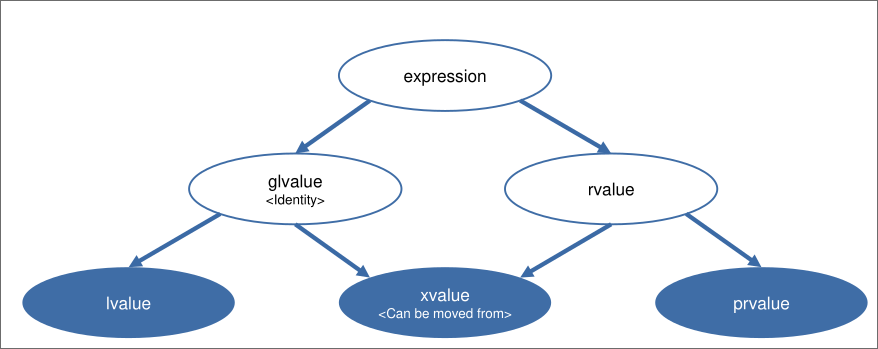
\includegraphics[scale=0.35]{2023_02_28_01_44_08.png}\newline
\begin{itemize}
\item \textcolor{purple}{lvalue}
  \begin{itemize}
  \item \textcolor{black}{address can be taken}
  \item \textcolor{black}{Can be on the left-hand side of an assignment if modifiable}
  \item \textcolor{black}{Can be used to initialize lvalue references}
  \item \textcolor{black}{Examples: variables, function calls that return reference, increment and decrement operators, array index access if array is lvalue}
  \item all string literals
  \end{itemize} 
\item \textcolor{purple}{prvalue}
  \begin{itemize}
  \item \textcolor{black}{address can't be taken -> doesn't exist}
  \item \textcolor{black}{cannot be on the left hand side of assignment}
  \item \textcolor{black}{temporary "materialization" to xvalue}
  \item \textcolor{black}{Examples: literals, false, nullptr, function call with non reference return type, postincrement and postdecrement!! }
  \end{itemize} 
\item \textcolor{purple}{xvalue}
  \begin{itemize}
  \item \textcolor{black}{address cannot be taken}
  \item \textcolor{black}{Cannot be used as left-hand operator of built-in assignment}
  \item \textcolor{black}{Conversion from prvalue through temporary materialization}
  \item \textcolor{black}{Examples: function calls with rvalue reference return type -> std::move, access of non-references members of an rvalue object, arra index access when array is rvalue}
  \end{itemize} 
\end{itemize}

\subsubsection{Temporary Materialization}
Getting from something imaginary to something you can point to....\newline
When this happens:\newline
\begin{itemize}
\item \textcolor{purple}{binding a reference to a prvalue}
\item \textcolor{purple}{when accessing a member of prvalue}
\item \textcolor{purple}{when accessing an element of a prvalue array}
\item \textcolor{purple}{when converting a prvalue array to a pointer}
\item \textcolor{purple}{when initializing an std::initializer\_list<T> from a braced-init-list}
\item \textcolor{red}{Type needs to be complete and needs to have a destructor}
\end{itemize} 
\begin{lstlisting}
struct Ghost {
  auto haunt() const -> void {
    std::cout << "booooo!\n";
  }
  //~Ghost() = delete;
};
auto evoke() -> Ghost {
  return Ghost{};
}
auto main() -> int {
  Ghost&& sam = evoke(); // bind reference to a prvalue
  Ghost{}.haunt(); // access member of prvalue
}
\end{lstlisting}

\subsection{l and rvalue references}
\begin{itemize}
\item \textcolor{purple}{lvalue reference} \textcolor{red}{made only of lvalues!!}
  \begin{itemize}
    \item type: T\&
  \item \textcolor{black}{alias for a variable}
  \item \textcolor{black}{can be used as function member type, local member/variable, return type}
  \item \textcolor{black}{be aware of dangling references when returning!}
  \end{itemize} 
\item \textcolor{purple}{rvalue reference} \textcolor{red}{made of rvalues, prvalues or xvalues!}
  \begin{itemize}
    \item \textcolor{black}{Type: T\&\&}
  \item \textcolor{black}{when assigned to a name (for example inside of a function), then it is actually an lvalue!!}
  \item \textcolor{black}{Argument is either a literal or a temporary object}\newline 
    \begin{lstlisting}
    std::string createGlass() -> std::string;
void fancyNameForFunction() { 
  std::string mug{"cup of coffee"};
  std::string&& glass_ref = createGlass(); //life-extension of temporary
  std::string&& mug_ref = std::move(mug); //explicit conversion lvalue to rvalue
  int&&
  i_ref = 5;
  //binding rvalue reference to prvalue
}
    \end{lstlisting}
  \end{itemize} 
\end{itemize} 

\subsection{Binds}
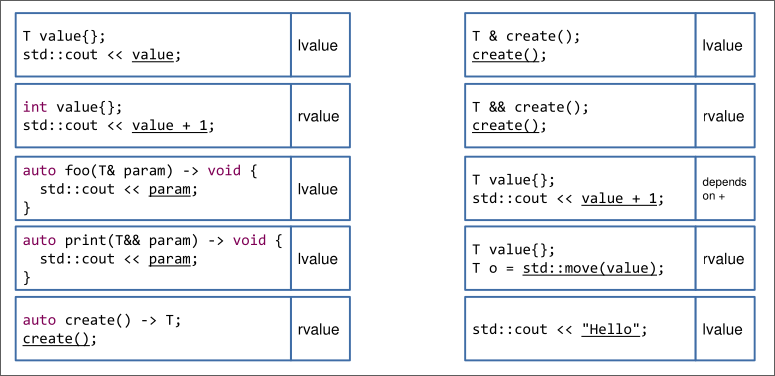
\includegraphics[scale=0.3]{2023_02_28_02_08_52.png}
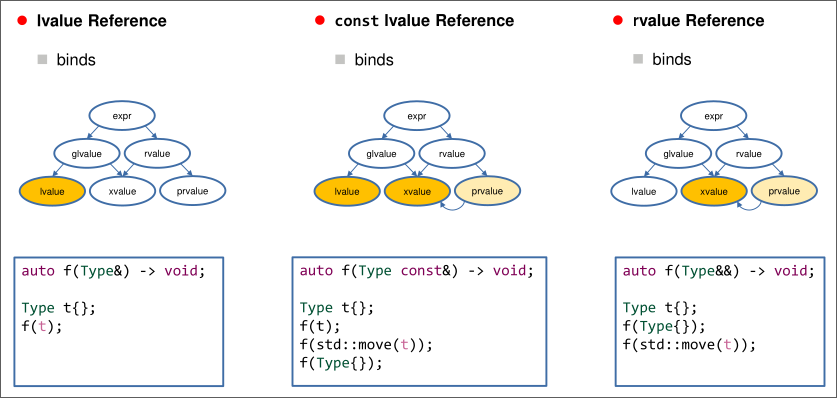
\includegraphics[scale=0.35]{2023_02_28_02_09_12.png}\newline
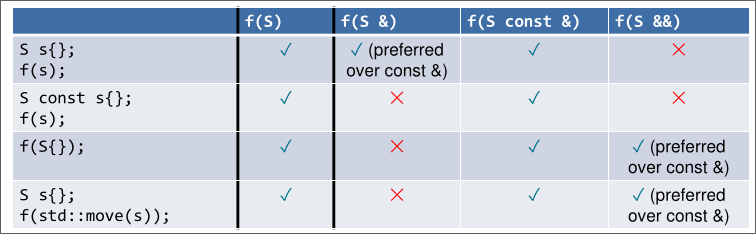
\includegraphics[scale=0.35]{2023_02_28_02_10_51.png}
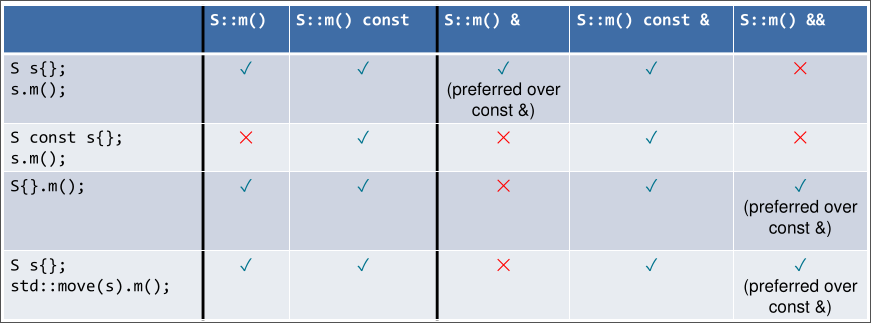
\includegraphics[scale=0.3]{2023_02_28_02_11_11.png}

\subsection{Destructor}
\textcolor{purple}{Whenever you need to write an explicit destructor, please make sure that you will not throw exeptions here. This can cause memory to not be freed, which.... well you guess what heppens}
\textcolor{teal}{In general you should make sure that \emph{ANY form of memory management doesn't throw exceptions!!!}}

\subsection{Default Constructors and user defined Constructors}
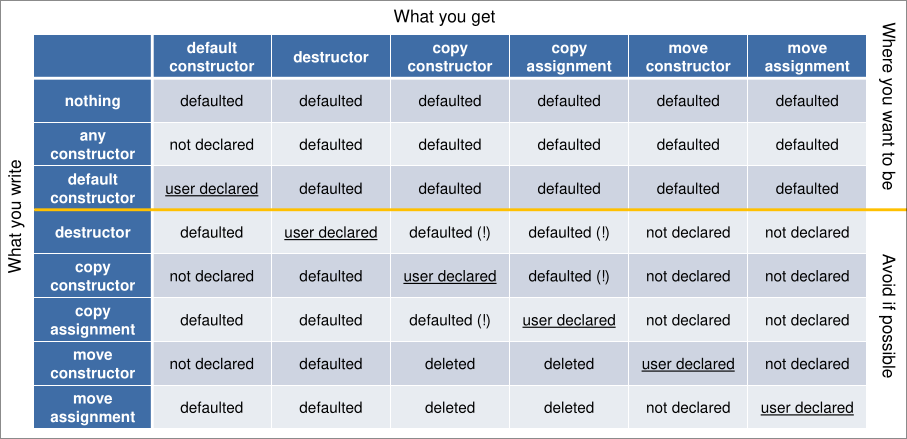
\includegraphics[scale=0.4]{2023_02_28_02_42_31.png}\newline
\textcolor{teal}{The ! means that it is a standard library bug, don't use those defaulted ones!!!}\newline
\textcolor{red}{Note that deleting a constructor will be the same as "user declared"!!}

\subsection{The problem with func(T const\&)}
\textcolor{purple}{When working with const T references, this implies that we can either \emph{copy or move it}, this means we will not necessarily know what we get.}\newline
\textcolor{teal}{The only possible way without type deduction is an overload for both.}
\begin{lstlisting}
template <typename T>
  auto log_and_do(T const& param) -> void {
  //log
  do_something(param);
} // lvalue 
template <typename T>
  auto log_and_do(T&& param) -> void {
  //log
  do_something(std::move(param));
} // lvalue and rvalue!!
\end{lstlisting}
\textcolor{red}{Note, with more parameters, you would need x amount of overloads for each combination of parameters!!}

\section{Type Deduction}

\subsection{Forwarding Reference}
\textcolor{purple}{A T\&\& is not always an rvalue! In some cases, it is a forwarding reference, which can be either an lvalue or an rvalue!!}\newline
\begin{lstlisting}
template <typename T>
auto f(T && param) -> void;

// lvalue
int x = 23;
f(x);
// auto f(int & param) -> void; (inferred)

// rvalue
f(23);
// auto f(int && param) -> void; (inferred)
\end{lstlisting}

\subsection{Rules for Type Deduction}
\begin{lstlisting}
// base function
template <typename T>
auto f(T param) -> void;

// type usages with function instances and deduced T
int          x = 23; // f(x) = f(int param) -> T = int
int const   cx = x; // f(cx) = f(int param) -> T = int
int const& crx = x; // f(crx) = f(int param) -> T = int
char const * const ptr = /* something */; // f(ptr) = f(char const * param) -> T = char const*;
// -- ignore outermost const
// -- ignore reference types
// -- take base type

// base function 2 
template <typename T>
auto f(T & param) -> void;

// type usages with function instances and deduced T
int          x = 23;  // f(x) = f(int& param) -> T = int
int const   cx = x;   // f(cx) = f(int const& param) -> T =int const
int const& crx = x;   // f(crx) = f(int const& param) -> T = int const
// -- ignore reference type

// base function 3
template <typename T>
auto f(T const& param) -> void;

// type usages with function instances and deduced T
int          x = 23; // f(x) = f(int const& param) -> T = int
int const   cx = x;  // f(cx) = f(int const& param) -> T = int
int const& crx = x;  // f(crx) = f(int const& param) -> T = int
// -- ignore reference types
// -- take base type

// base function 4
template <typename T>
auto f(T&& param) -> void;

// type usages with function instances and deduced T
int          x = 23; // f(x) = f(int& param) -> T = int&
int const   cx = x;  // f(cx) = f(int const& param) -> T = int const&
int const& crx = x;  // f(crx) = f(int const& param) -> T = int const&
//                   // f(27) = f(int&& param) -> T = int 
// -- if param is an lvalue, then they become lvalue references
// -- otherwise rvalue, default rules for references

\end{lstlisting}

\subsubsection{Deducing Initializer Lists}
\textcolor{purple}{With initializer lists, you can't directly deduce the type as it will think T is the entire list, which is nonsense!}
\begin{lstlisting}
template <typename T>
auto f(T param) -> void;
f({23}); //error

template <typename T>
auto f(std::initializer_list<T> param) -> void;
f({23}); //T = int
//ParamType = std::initializer_list<int>
\end{lstlisting}

\subsubsection{Deducing auto types}
\begin{lstlisting}
autox = 23;         //auto is a value type
auto const cx = x;  //auto is a value type
auto& rx = x;       //auto is a reference type
auto&& uref1 = x;   //x is an lvalue, uref1 is int&
auto&& uref2 = cx;  //cx is an lvalue, uref2 is int const&
auto&& uref3 = 23;  //23 is an rvalue, uref3 is int&&

// special cases
auto init_list1 = {23};  //std::initializer_list<int>
auto init_list2{23};     //int, was std::initializer_list<int>
auto init_list3{23, 23}; //Error, requires one single argument
\end{lstlisting}
\textcolor{purple}{Note that auto type deduction works with parameters and return types, with the special cases like initializer list still applying!!}

\subsubsection{Type Deduction with Decltype}
\begin{lstlisting}
int           x       = 23;
int const     cx      = x;
decltype(cx)  cx_too  = cx; //type of cx_too is int const
int&          rx      = x;
decltype(rx)  rx_too  = rx; //type of rx_too is int&

// these two are the only surprises! auto only gives the base type without reference, while the other gives the full reference type
auto just_x = rx; //type of just_x is int
decltype(auto) more_rx = rx; //type of more_rx is int&
\end{lstlisting}
\textcolor{orange}{decltype(auto) etc can also be used for returning something specific:} 
\begin{lstlisting}
// auto decltype
template <typename Container, typename Index>
decltype(auto) access(Container & c, Index i) {
  return c[i];
}

// specific decltype
template <typename Container, typename Index>
auto access(Container & c, Index i) -> decltype(c[i]) {
  return c[i];
}
\end{lstlisting}
\textcolor{red}{Note we can only declare decltype(c[i]) as a trailing type! The reason for this is that c and i are only known AFTER the parameters!}

\subsubsection{Returns with decltype}
\begin{lstlisting}
decltype(auto) funcName() {
  int local = 42;
  return local; // decltype(local) => int
} // lvalue -> T
decltype(auto) funcNameRef() {
  int local = 42;
  int & lref = local;
  return lref; // int & -> bad (dangling)
} // lvalue reference -> T&
decltype(auto) funcXvalue() {
  int local = 42;
  return std::move(local); // int && -> bad (dangling)
} // rvalue reference -> T&&
decltype(auto) funcLvalue() {
  int local = 42;
  return (local); // int & -> bad (dangling)
} // lvalue reference -> T&
decltype(auto) funcPrvalue() {
  return 5; // int
} // prvalue -> T
\end{lstlisting}

\subsection{Checking for r and l-values}
\textcolor{purple}{We learned that we can solve the issue of multiple overloads with T\&\&, but what if we want to differentiate after the fact? std::forward!}
\begin{lstlisting}
template <typename T>
auto log_and_do(T&& param) -> void {
  //log
  do_something(std::forward<T>(param));
}

// example for implementation
template <typename T>
  decltype(auto) forward(std::remove_reference_t<T>& param) {
  return static_cast<T&&>(param);
}
// explanation
// this will check if we have an lvalue or not by trying to cast to an rvalue reference
// if & and && are casted, it will always result in &
// this means only an rvalue will result in an rvalue being returned, everything else will result in lvalue being returned
// this is called reference collapsing!
// example -> when T is int& the static cast will be int& && and hence collapsed to int&
// when T is int&& the static cast will be int&& && and hence collapsed to int&&
// when T is int, the static cast will be int&&, no collapse is needed here.
// note references are only checked for the type, the actual references are removed, as can be seen by the std::remove_reference_t
\end{lstlisting}
\textcolor{orange}{This means that forwards is essentially \emph{a conditional cast to an rvalue reference!}}\newline
Rules for reference collapsing:
\begin{itemize}
  \item \textcolor{purple}{\& and \& = \&}
  \item \textcolor{purple}{\&\& and \& = \&}
  \item \textcolor{purple}{\& and \&\& = \&}
  \item \textcolor{purple}{\&\& and \&\& = \&\&}
\end{itemize} 

\subsubsection{std::move vs std::forward}
\textcolor{purple}{While forward is the \emph{conditional cast}, std::move is the \emph{unconditional cast}! This means you will always receive an rvalue!}
\begin{lstlisting}
// std::forward
template <typename T>
  decltype(auto) forward(std::remove_reference_t<T>& param) {
  return static_cast<T&&>(param); 
} // will collapse dynamically
// std::move
template <typename T>
decltype(auto) move(T&& param) { // param is always T&& !!!
  return static_cast<std::remove_reference_t<T>&&>(param);
} // will always collapse to && and && meaning && is returned
\end{lstlisting}

\section{Lambdas}

\subsection{From lambda to actual code}
\begin{lstlisting}
// lambda
int i0 = 42;
auto missingMutable = [i0] {return i0++;};

// compiler code
struct CompilerKnows {
  auto operator()() const -> int {
    return i0++;
  }
  int i0;
};
\end{lstlisting}

\section{Memory Management and Heap}

\subsection{Pointers}
Funny pointer consty fun.\newline
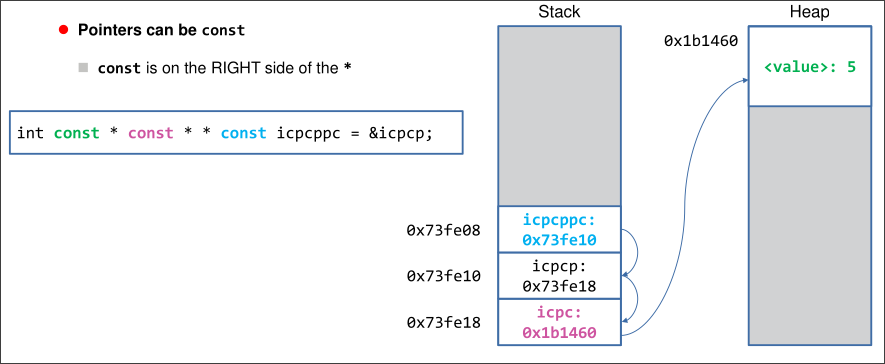
\includegraphics[scale=0.4]{2023_03_21_01_51_22.png}

\subsubsection{Reading a pointer declaration}
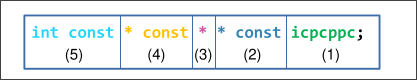
\includegraphics[scale=0.4]{2023_03_21_02_11_12.png}
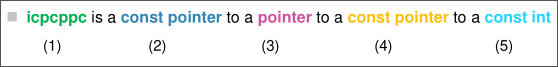
\includegraphics[scale=0.4]{2023_03_21_02_11_17.png}
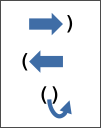
\includegraphics[scale=0.4]{2023_03_21_02_11_21.png}\newline
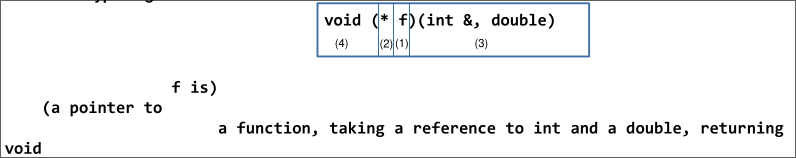
\includegraphics[scale=0.4]{2023_03_21_02_13_39.png}\newline
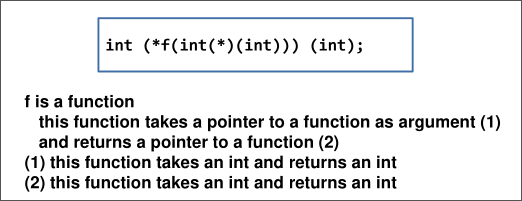
\includegraphics[scale=0.4]{2023_03_21_02_15_03.png}
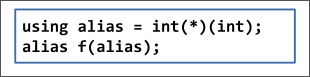
\includegraphics[scale=0.4]{2023_03_21_02_16_22.png}

\subsubsection{nullptr}
\textcolor{teal}{The nullptr has a more specific meaning than either 0 or NULL, \newline
other than 0, it has no implicit conversion to integral type, unlike 0, and also ensures no mistakes with overloads -> again integral.}\newline
\textcolor{red}{There is also the implicit conversion from nullptr to T*}
\begin{lstlisting}
int* test = nullptr;
float* test2 = nullptr;

// lol
void* something = nullptr;
int* no = (int*) something;
\end{lstlisting}

\subsection{Const}
By default the const keyword needs to be on the right, the only exception is the first type on the left!\newline
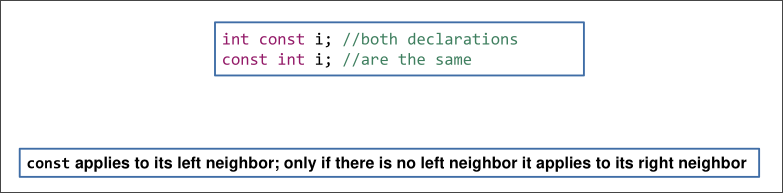
\includegraphics[scale=0.4]{2023_03_21_02_16_58.png}\newline
\textcolor{red}{Be careful with left const assignments when using aliases!}
\begin{lstlisting}
// Extract the int const * part
using alias = int const *;
alias const icpc; // works well

// Extract the int * const part
using alias = int * const;
const alias cipc; // this is bs! Compiles however!
\end{lstlisting}

\subsection{mutable}
\textcolor{teal}{The mutable keyword is always used on the variable itself!}
\begin{lstlisting}
// the value at mutable_const_int_pointer is constant
// however the pointer itself is not!
// the mutable keyword here is only used for const functions -> can be used inside of them
class Something {
  mutable const int * mutable_const_int_pointer;
}
\end{lstlisting}

\subsection{New}
\begin{lstlisting}
struct Point {
  Point(int x, int y):x {x}, y {y}{}
  int x, y;
};
auto createPoint(int x, int y) -> Point* {
  return new Point{x, y}; //constructor
}
auto createCorners(int x, int y) -> Point* {
  return new Point[2]{{0, 0}, {x, y}};
}
\end{lstlisting}

\subsection{Delete}
\textcolor{teal}{Every new needs to be accomodated with a delete, \emph{deleting twice will lead to undefined behavior!}.}\newline
\textcolor{purple}{However, deleting the nullptr is well defined, it does nothing.}
\begin{lstlisting}
struct Point {
  Point(int x, int y):x {x}, y {y} {}
  int x, y;
}
auto funWithPoint(int x, int y) -> void {
  Point * pp = new Point{x, y};
  //pp member access with pp->
  //pp is the pointer value
  delete pp; //destructor
}
\end{lstlisting}
Using delete with [] will delete arrays. 
\begin{lstlisting}
struct Point {
  Point(int x, int y) :x {x}, y {y}{}
  int x, y;
}
auto funWithPoint(int x, int y) -> void {
  Point * arr = new Point[2]{{0, 0},{x, y}};
  //element access with [], e.g. arr[1]
  //arr points to the first element
  delete[] arr; //destructors
} // this also deletes multidimensional arrays!!
\end{lstlisting}

\subsubsection{Placement new}
\textcolor{purple}{This takes a ptr where \emph{currently no element is placed} and creates a new class instance of choice in this pointer.\newline
This means that you can potentially create a pointer to a smaller instance. It just needs to be suitable, aka big enough, so bigger objects won't work!!}
\begin{lstlisting}
struct Point {
  Point(int x, int y):x {x}, y {y}{}
  int x, y;
};
auto funWithPoint() -> void {
  auto ptr = new Point{9, 8};
  // must release Point{9, 8}
  // release can be done with ptr->~NewTest();
  // or with std::destroy_at(ptr);
  new (ptr) Point{7, 6};
  delete ptr;
}
\end{lstlisting}

\subsubsection{Placement Destroy}
\textcolor{purple}{There is no proper placement destroy, instead there is the \emph{regular destructor, but that one doesn't work with primitive built-in types,\newline
so instead use std::destroy\_at.}}
\begin{lstlisting}
struct Resource {
  Resource() {
    /*allocate resource*/
  }
  ~Resource() {
    /*deallocate resource*/
  }
};
auto funWithPoint() -> void {
  auto ptr = new Resource{};
  ptr->~Resource();
  new (ptr) Resource{};
  delete ptr;
}
\end{lstlisting}

\subsubsection{Non Default Constructible Types}
\textcolor{purple}{This refers to types that do not have a constructor with no parameters. -> defualt constructor\newline
With these types we can't use new TypeName, instead we need to allocate memory explicitly like this:}
\begin{lstlisting}
struct Point {
  Point(int x, int y); // default deleted!
  ~Point();
  int x, y;
};

// allocate memory
auto memory = std::make_unique<std::byte[]>(sizeof(Point) * 2);

// initialize
new (memory.get()) Point{1, 2};
\end{lstlisting}
\textcolor{purple}{Accessing these individually is tedious, how about e helper?}
\begin{lstlisting}
auto elementAt(std::byte * memory, size_t index) -> Point& {
  return reinterpret_cast<Point *>(memory)[index];
}

auto memory = std::make_unique<std::byte[]>(sizeof(Point * 2));
Point * first = &elementAt(memory.get(), 0);
new (first) Point{1, 2};
Point * second = &elementAt(memory.get(), 1);
new (second) Point{4, 5};

// make sure to also destroy it manually!
// it ain't rust so get shit on
// order is irrelevant for the memory management itself.
std::destroy_at(second);
std::destroy_at(first);
\end{lstlisting}
\textcolor{red}{You have to destroy the memory manually however!\newline
\emph{The reason for this is that each object might have heap allocated memory itself, this is NOT guaranteed to be cleaned up.}}

\subsubsection{New and Delete are fucking operators...}
\begin{lstlisting}
struct not_on_heap {
  static auto operator new(std::size_t sz) -> void * {
    throw std::bad_alloc{};
  }
  static auto operator new[](std::size_t sz) -> void * {
    throw std::bad_alloc{};
  }
  static auto operator delete(void *ptr) -> void noexcept {
    // do nothing, never called, but should come in pairs
  }
  static auto operator delete[](void *ptr) -> void noexcept {
    // do nothing, never called, but should come in pairs
  }
  // just no
  // but you can create your own allocators
  // or simply make sure that noone ever calls new or delete with your types, kekw
};
\end{lstlisting}

\subsubsection{Typical Problems with memory}
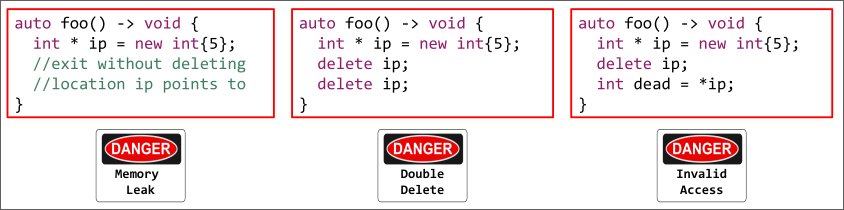
\includegraphics[scale=0.4]{2023_03_21_03_06_31.png}\newline
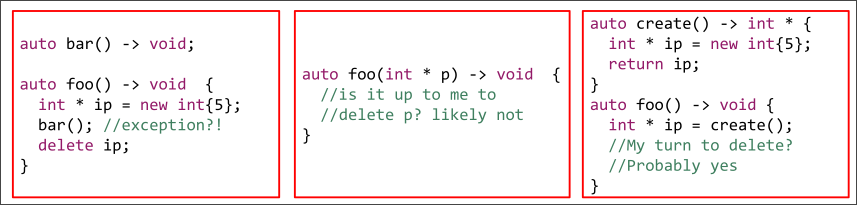
\includegraphics[scale=0.4]{2023_03_21_03_06_47.png}

\section{Static vs Dynamic Polymorphism}
\subsection{Static}
\begin{itemize}
\item \textcolor{black}{faster at runtime}\newline
  no need to ckeck or cast function, just use it
\item \textcolor{black}{slower at compile time }\newline
  each implementation used will be made with macros
\item \textcolor{black}{syntax checking is off -> lsp limitation in c++}
\item larger binaries -> more code
\end{itemize} 

\subsection{Dynamic}
The problem is displayed as follows: 
\begin{lstlisting}
struct Shape {
  virtual unsigned area() const = 0;
  virtual ~Shape();
};
struct Square : Shape {
  Square(unsigned side_length)
  : side_length{side_length} {}
  unsigned area() const {
    return side_length * side_length;
  }
  unsigned side_length;
};

decltype(auto) amountOfSeeds(Shape const & shape) {
  auto area = shape.area();
  return area * seedsPerSquareMeter;
};
\end{lstlisting}
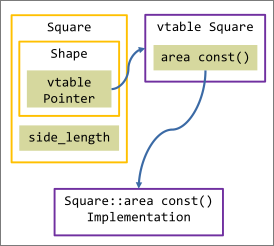
\includegraphics[scale=0.4]{2023_04_04_01_26_12.png}\newline
\textcolor{teal}{The problem is that we need to cast when using these functions. 
Once again you can see the shit that is inheritance as it forces this conveluted casting style of writing code.}

\subsubsection{Comparison to static}
\begin{lstlisting}
struct Square {
  Square(unsigned side_length)
  : side_length{side_length} {}
  unsigned area() const {
    return side_length * side_length;
  }
  unsigned side_length;
};

template<typename ShapeType>
decltype(auto) amountOfSeeds(ShapeType const & shape) {
  auto area = shape.area();
  return area * seedsPerSquareMeter;
}

// instance -> not written by programmer -> made by compiler
// decltype(auto) amountOfSeeds(Square const & shape) {
//   auto area = shape.area();
//   return area * seedsPerSquareMeter;
// };
\end{lstlisting}
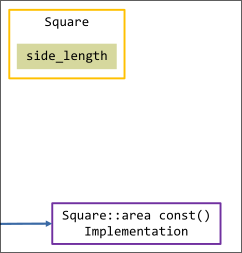
\includegraphics[scale=0.4]{2023_04_04_01_28_58.png}\newline
\textcolor{teal}{The only downside it that you can't use this with dynamic types, but once again this is why you don't use this crap.
Remember the pain that was in your rust game, the same thing would happen here.}

\subsubsection{Dynamic Dispatch Virtual Table}
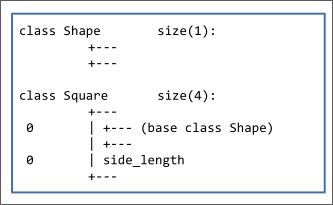
\includegraphics[scale=0.4]{2023_04_04_01_33_59.png}
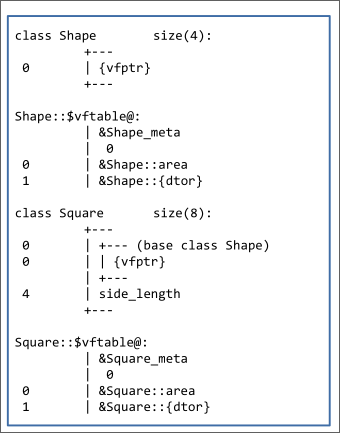
\includegraphics[scale=0.4]{2023_04_04_01_34_08.png}\newline
Note that the size(1) in the first figure is simply there, because in C++ each object needs to be differentiable.\newline
This means that you need some sort of address to do that. If this object doesn't actually exist, then there will be no size, as can be seen in the square.

\section{Substitution Failure}
The template itself does not throw a compilation error, meaning that if the template itself can't be done with a specific type, then we simply ignore the type for this template.
However, if we then go ahead and use this function somewhere and this specific type didn't work with this function, then we will receive a compiler error.
This is also the reason why the lsp is so bad at showing errors when it comes to templates.

\begin{lstlisting}
template <typename T>
auto increment(T value) -> T {
  return value.increment();
} // here string is just not considered as string has no .increment

increment("pingpang"); // error bro
\end{lstlisting}
\textcolor{teal}{You can use the dropping of instances of templates by using functions that only work on certain types in order to protect against using with strange types.}

\subsection{Type Traits}
\textcolor{teal}{Compares two types according to traits}\newline
\textcolor{red}{Note: These only work in \emph{Templates, Parameters and Return Types}, NOWHERE else!}
\begin{lstlisting}
template <typename T, typename U>
struct is_same : false_type {
  // inherits
  // static constexpr bool value = false;
};
template <typename T>
struct is_same<T, T> : true_type {
  // inherits
  // static constexpr bool value = true;
};
template <typename T, typename U>
constexpr bool is_same_v = is_same<T, U>::value;
\end{lstlisting}
\begin{itemize}
\item \textcolor{black}{std::is\_same<T,U>} compares the 2 types
\item \textcolor{black}{std::is\_same\_v<T,U>} same but results in bool -> ::value
\item \textcolor{black}{std::is\_same\_t<T,U>} same but results in type -> ::type
\item \textcolor{black}{std::is\_class<T>} Checks to see if type is a class type 
\item \textcolor{black}{std::is\_same\_v<T>} same but results in bool -> ::value 
\item \textcolor{black}{std::negation\_v<T>} negates the value 
\item \textcolor{black}{std::is\_reference<T>} checks if type is a reference type 
\item \textcolor{black}{std::is\_constructible\_v<T>} checks if compiler is constructible 
\end{itemize} 
\begin{lstlisting}
#include <type_traits>

struct S{};

auto main() -> int {
  std::is_class<S>::value; // true
  std::is_class<int>::value; // false
}
\end{lstlisting}
\begin{itemize}
\item \textcolor{black}{std::enable\_if<bool, T>} checks if type is of given type
\item \textcolor{black}{std::enable\_if\_t<bool, T>} -> ::type
\end{itemize} 
\begin{lstlisting}
template <bool expr, typename T = void>
struct enable_if{
  template <bool expr,typename T = void>
  struct enable_if{};

  template <typename T>
  struct enable_if<true, T> {
    using type = T;
  };

  template <bool expr,typename T = void>
  using enable_if_t = typename enable_if<expr, T>::type;
};

auto main() -> int {
  std::enable_if_t<true, int> i;      // int
  std::enable_if_t<false, int> error; // no type
}
\end{lstlisting}
\textcolor{teal}{Possibilities of application:}\newline
\begin{lstlisting}
template <typename T>
auto increment(T value) -> std::enable_if_t<std::is_class_v<T>, T> {
  return value.increment();
}

template <typename T>
auto increment(std::enable_if_t<std::is_class_v<T>, T> value) -> T {
  return value.increment();
} // enable_if as parameter, impairs type deduction

template <typename T, typename = std::enable_if_t<std::is_class_v<T>, void>>
auto increment(T value) {
  return value.increment();
} // would be void per default
\end{lstlisting}

\subsubsection{Constructors and type checks}
\begin{lstlisting}
template <typename T>
struct Box {
  Box() = default;
  template <typename BoxType, typename = std::enable_if_t<std::is_same_v<Box, BoxType>>>
  explicit Box(BoxType && other)
  : items(std::forward<BoxType>(other).items) {}
  // only matches when entered type can be made into .items
  explicit Box(size_t size)
  : items(size) {}
  //...
  private:
    std::vector<T> items{};
};
\end{lstlisting}
\textcolor{teal}{The problem is that with forward, the matching gets \emph{eager}, this means that int would match to the BoxType \&\& other, resulting in an error since int doesn't have .items}\newline
\textcolor{red}{This is just an example, do not use this over proper copy and move constructors}

\section{Requires C++20}
\textcolor{teal}{This is the solution to the previously complicated way of handling template type requirements}\newline
It can be done in these two ways:
\begin{lstlisting}
// after template, works for structs, classes and functions
template<typename T>
requires true // or anything that can resolve to bool
auto function(T argument) -> void {}

// after return type, only works for functions
template<typename T>
auto function(T argument) -> void requires true {} 


// explicit example
template <typename T>
requires std::is_class_v<T>
auto function(T argument) -> void {}
\end{lstlisting}

\subsection{Requires as function}
Sequence of actions: 
\begin{lstlisting}
requires {
  // Sequence of requirements
}
\end{lstlisting}
Requires with parameters:
\begin{lstlisting}
requires ($parameter-list$) {
  // Sequence of requirements
}
\end{lstlisting}
Example: 
\begin{lstlisting}
template <typename T>
requires requires (T const v) { v.increment(); }
auto increment(T value) -> T {
  return value.increment();
}
// yes, you need two requires.....
\end{lstlisting}

\subsection{Subtype Requirements}
\begin{lstlisting}
template<typename T>
requires {
  typename BoundedBuffer<T>::value_type;
  typename BoundedBuffer<T>::size_type;
  typename BoundedBuffer<T>::reference;
  typename BoundedBuffer<T>::const_reference;
}
\end{lstlisting}

\subsection{Compund Requirements}
\begin{lstlisting}
template <typename T>
requires requires (T const v) {
  { v.increment() } -> std::same_as<T>;
} // check if the return of the check to v.increment type == T
auto increment(T value) -> T {
  return value.increment();
}
\end{lstlisting}

\subsection{Concept Keyword}
\textcolor{teal}{These are essentially just traits...}
\begin{lstlisting}
template <typename T>
concept Incrementable = requires (T const v) { 
  {
    v.increment()
  } -> std::same_as<T>;
}; // potential to use || or && to chain requires!!
\end{lstlisting}

\subsubsection{Usage}
These are the same:
\begin{lstlisting}
template <Incrementable T>
auto increment(T value) -> T {
  return value.increment();
}

template <typename T>
requires Incrementable<T>
auto increment(T value) -> T {
  return value.increment();
}
\end{lstlisting}

\subsection{AutoTemplates}
You can use the auto keyword to automatically use templates:
\begin{lstlisting}
// both are the same
auto function(auto argument) -> void {}

template <typename T>
auto function(T argument) -> void {}
\end{lstlisting}

\subsubsection{Problems with auto templates}
\begin{lstlisting}
auto function(auto arg1, auto arg1) -> void {}

// ignored!!!!
template <typename T>
auto function(T arg1, T arg2) -> void {}

// chosen, the auto automatically converts to this
template <typename T1, typename T2>
auto function(T1 arg1, T2 arg2) -> void {}
\end{lstlisting}

\subsubsection{Concept with auto}
\begin{lstlisting}
// both are the same
auto increment(Incrementable auto value) -> T {
  return value.increment();
}

template <Incrementable T>
auto increment(T value) -> T {
  return value.increment();
}
\end{lstlisting}

\section{Compile Time Evaluation}

\subsection{Legacy}
global const variables are essentially the same thing as const in rust -> evaluated at compile time.
\begin{lstlisting}
size_t const SZ = 6 * 7; // evaluated during compilation
double x[SZ]; // -> x == SZ
\end{lstlisting}

\subsection{Constant Expression Contexts}
These are the contexts where compile time evaluation is possible:
\begin{itemize}
\item \textcolor{black}{non-type template arguments}\newline
  \begin{lstlisting}
  std::array<Element, 5> arr{}
  \end{lstlisting}
\item \textcolor{black}{array bounds}\newline
  \begin{lstlisting}
  double matrix[ROWS][COLS]{}
  \end{lstlisting}
\item \textcolor{black}{Case expressions}\newline
  \begin{lstlisting}
  switch(value) {
  case 42: // ...
  }
  \end{lstlisting}
\item \textcolor{black}{Enumerator Initializer}\newline
  \begin{lstlisting}
  enum Light {
  Off = 0, On = 1
  };
  \end{lstlisting}
\item static\_assert \newline
  \begin{lstlisting}
  static_assert(order == 66);
  \end{lstlisting}
\item constexpr variables\newline
  \begin{lstlisting}
  constexpr unsigned pi = 3;
  \end{lstlisting}
\item constexpr if statements\newline
  \begin{lstlisting}
  if constexpr (size > 0) {
  // ..
  }
  \end{lstlisting}
\item noexcept\newline
  \begin{lstlisting}
  Blob(Blob &&) noexcept(true);
  \end{lstlisting}
\end{itemize} 

\subsection{static\_assert}
Can be used to check things on compile time -> e.g. tests during compile time.\newline
\textcolor{teal}{Note, the compilation fails if the assert fails!}
\begin{lstlisting}
// usage: static_assert(condition, message(optional))
static_assert(isGreaterThanZero(Capacity));
static_assert(sizeof(int) == 4, "unexpected size of int");
\end{lstlisting}

\subsection{constexpr/constinit}
variables evaluated at compile time -> literal values 5,6,"asdf",constexpr functions.
\begin{lstlisting}
constexpr unsigned pi = 3;
constinit unsigned pi = 3;
\end{lstlisting}
\begin{itemize}
\item \textcolor{black}{scopes}\newline
  local, namespace, global -> static
\item \textcolor{black}{constexpr variables are const}
\item \textcolor{black}{constinit variables are not const!}
\end{itemize} 

\subsection{constexpr functions}
\textcolor{red}{Can't use exceptions, which are shit either way!}\newline
Functions that are evaluated at compile time:
\begin{lstlisting}
constexpr auto factorial(unsigned n) {
//...
}
\end{lstlisting}
\textcolor{teal}{Note, these functions can only have variables of literal type, and these MUST be initialized before used.}\newline
You can also:
\begin{itemize}
\item \textcolor{black}{use loops}
\item \textcolor{black}{branches -> if can be evaluated at compile time -> no exceptions!}
\item \textcolor{black}{can only call constexpr functions}
\item allocate new memory with new,delete or unique pointers etc.
\item use constexpr functions as virtual functions in classes and structs
\end{itemize} 
\textcolor{teal}{Note that you can use constexpr in non constexpr contexts, in this case it will try to evaluate this constexpr at compile time if possible}

\subsubsection{Consteval}
These are essentially the same thing as constexpr functions, but they will \emph{always} evaluate at compile time, this means it can only be used in constexpr contexts.
\begin{lstlisting}
consteval auto factorial(unsigned n) {
  auto result = 1u;
  for (auto i = 2u; i <= n; i++) {
    result *= i;
  }
  return result;
}
constexpr auto factorialOf5 = factorial(5);
auto main() -> int {
  static_assert(factorialOf5 == 120);
}
\end{lstlisting}

\subsection{Undefined behavior and compiler}
\textcolor{teal}{Interestingly enough the compiler will prevent undefined behavior in the compilation itself, instead it will just stop the compilation and return an errormessage.}\newline
Note that for compile time evaluations, should code not actually reach invalid code, then it will just work, since that code was not reached.... another template fun thing with c++...
\begin{lstlisting}
constexpr auto throwIfZero(int value) -> void {
  if (value == 0) {
    throw std::logic_error{""};
  }
}
constexpr auto divide(int n, int d) -> int {
  throwIfZero(d);
  return n / d;
}
constexpr auto five = divide(120, 24);
// this is not reached, if it would be then it would not compile
constexpr auto failure = divide(120, 0);
\end{lstlisting}

\subsection{Literal Types}
\begin{itemize}
\item \textcolor{black}{Trivial Destructor}
\item \textcolor{black}{special literal types:}\newline
  \begin{itemize}
  \item \textcolor{black}{Lambdas}
  \item \textcolor{black}{References}
  \item \textcolor{black}{Arrays of Literal Types}
  \item \textcolor{black}{void}
  \item int, double, pointers, enums, literal strings, strings, etc.
  \end{itemize} 
\end{itemize} 
\textcolor{teal}{You can create your own literal type:}
\begin{lstlisting}
template <typename T>
class Vector {
  constexpr static size_t dimensions = 3;
  std::array<T, dimensions> values{};
  public:
  constexpr Vector(T x, T y, T z)
  : values{x, y, z}{}
  constexpr auto length() const -> T {
    auto squares = x() * x() +
    y() * y() +
    z() * z();
    return std::sqrt(squares);
  }
  constexpr auto x() -> T& {
    return values[0];
  }
  constexpr auto x() const -> T const& {
    return values[0];
  }
  //...
};
\end{lstlisting}
\begin{itemize}
\item \textcolor{red}{at least one constexpr or consteval constructor}
\item \textcolor{red}{trivial destructor}
\item \textcolor{red}{const and non-const functions possible}
\item \textcolor{red}{note that only constexpr or consteval functions are done at compile time!}
\item \textcolor{red}{Can be a template}
\item \textcolor{red}{Other functions don't \emph{need} to be constexp or consteval!}
\end{itemize} 

\subsubsection{Compile Time template class computation}
\begin{lstlisting}
template <size_t n>
struct fact {
  static size_t const value{(n > 1)?
};
n * fact<n-1>::value : 1};
  template <>
  struct fact<0> { // recursion base case: template specialization
  static size_t const value = 1;
};
TEST(testFactorialCompiletime) {
  constexpr auto result = fact<5>::value;
  ASSERT_EQUAL(result, 2 * 3 * 4 * 5);
}
\end{lstlisting}

\subsubsection{Captures in Lambdas are also literal types}
\begin{lstlisting}
constexpr auto cubeVolume(double x) {
  // x is literal
  auto area = [x] {return pi * x * x;};
  return area() * x;
}
constexpr auto cV = cubeVolume(5.0);
\end{lstlisting}

\subsubsection{Variable declaration as templates}
\begin{lstlisting}
template <size_t N>
constexpr size_t factorial = factorial<N - 1> * N;

template <> //Base case
constexpr size_t factorial<0> = 1;

// the idea is that you can have recursive variable declarations.... wtf?
\end{lstlisting}

\subsection{User Defined Literal-Suffixes}
\subsubsection{Problem}
\begin{lstlisting}
template <typename Unit>
struct Speed {
  constexpr explicit Speed(double value)
  : value{value}{};
  constexpr explicit operator double() const {
    return value;
  }
  private:
  double value;
};
\end{lstlisting}
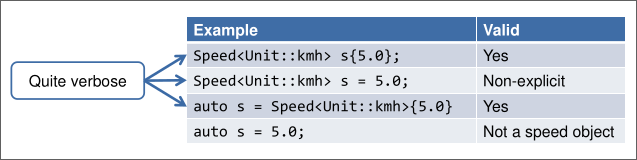
\includegraphics[scale=0.4]{2023_04_18_02_29_26.png}


\subsubsection{Solution}
\textcolor{teal}{This is basically an overload on a literal ending → This means you can create something like numbers with endings like kph, kilo or whatever you need.}\newline
In order to achieve this, you need to overload the "" operator ending with your literal.\newline
Also note, \textcolor{teal}{The literal needs to be in a namespace in order to avoid confusion.}\newline
This suffix should only have these literals inside of it, nothing else!
\begin{lstlisting}
namespace velocity::literals {
  constexpr inline auto operator"" _kph(unsigned long long value) -> Speed<Kph> {
    return Speed<Kph>{safeToDouble(value)};
  }
  constexpr inline auto operator"" _kph(long double value) - Speed<Kph> {
    return Speed<Kph>{safeToDouble(value)};
  }
  auto speed1 = 5.0_kph;
  auto speed2 = 5.0_mph;
  auto speed3 = 5.0_mps;
}
\end{lstlisting}
This version is used to avoid wrappers that add a lot of boilerplate code and makes it hard to use as you need to unwrap the wrappers.
\textcolor{red}{Note, you can only overload a set of types -> (unsigned long long), (char const* , std::size\_t), (char const *)\newline
I assume only literal types???}

\subsubsection{String as suffix}
\begin{lstlisting}
auto operator"" _suffix(char const *, std::size_t len) -> TYPE

namespace mystring {
  inline auto operator"" _s(char const *s, std::size_t len) -> std::string {
    return std::string { s, len };
  }
}
// ...
using namespace mystring;
auto s = "hello"_s;
s += " world\n";
std::cout << s;
\end{lstlisting}
Or you can convert integers and floats to string: 
\begin{lstlisting}
auto operator"" _suffix(char const *) -> TYPE

// this takes the non 0 terminated strings
namespace mystring {
  inline auto operator"" _s(char const *s) -> std::string
    return std::string { s };
  }
}
\end{lstlisting}
\textcolor{red}{Note, these can't be constexpr!}

\subsubsection{Compile Time User Defined Suffixes}
\begin{lstlisting}
// variadic version of suffix operator
template <char ...Digits> requires (is_ternary_digit(Digits) && ...)
constexpr auto operator"" _ternary() -> unsigned long long {
  return ternary_value<Digits...>;
}

constexpr auto three_to(std::size_t power) -> unsigned long long {
  return power ? 3ull * three_to(power - 1) : 1ull;
}

template <char ...Digits>
extern unsigned long long ternary_value;

// handle 0
template <char ...Digits>
constexpr unsigned long long ternary_value<'0', Digits...> {
  ternary_value<Digits...>
};

// handle 1
template <char ...Digits>
constexpr unsigned long long ternary_value<'1', Digits...> {
  1 * three_to(sizeof ...(Digits)) + ternary_value<Digits...>
};

// handle 2 
template <char ...Digits>
constexpr unsigned long long ternary_value<'2', Digits...> {
  2 * three_to(sizeof ...(Digits)) + ternary_value<Digits...>
};

// handle base case
template<>
constexpr unsigned long long ternary_value<>{0};
\end{lstlisting}
\textcolor{teal}{Newer versions of c++ also allow a more concise version}
\begin{lstlisting}
constexpr auto is_ternary_digit(char c) -> bool {
  return c == '0' || c == '1' || c == '2';
}
constexpr auto value_of(char c) -> unsigned {
  return c - '0';
}
template <char D, char ...Digits>
constexpr ternary_value<D, Digits...> {
  value_of(D) * three_to(sizeof ...(Digits)) + ternary_value<Digits...>
};
\end{lstlisting}

\subsubsection{Default Suffixes}
\begin{itemize}
\item \textcolor{black}{string -> s}
\item \textcolor{black}{std::complex -> i,il,if (imaginary numbers)}
\item \textcolor{black}{std::chrono::duration -> ns,us,ms,s,min,h (time)}
\end{itemize} 

\section{Multithreading and Mutexes}

\subsection{std::thread}
This is a replacement for the POSIX API which is rather dated, and does not lead to clean code.\newline
It mostly works, but some things need to fall back to POSIX, or microtroll API on windoof.

\begin{lstlisting}
#include <thread>

auto main() -> int {
  // just like in rust -> create thread with closure/lambda
  std::thread greeter {
    [] { std::cout << "Hello, I'm thread!" << std::endl; }
  };
  // join the main thread -> blocking
  greeter.join();
}
\end{lstlisting}

\subsubsection{Functors}
You can also use a struct/class as parameter to pass into the std::thread.\newline
This essentially means defining a struct with the function operator()() -> which essentially means turning it into a lambda with data attached.\newline
\begin{lstlisting}
#include <thread>

struct Functor {
  auto operator()() const -> void {
    std::cout << "Functor" << std::endl;
  }
};

auto function() -> void {
  std::cout << "Function" << std::endl;
  // return value ignored -> aka only void supported
}

auto main() -> int {
  std::thread functionThread{function};
  std::thread functorThread{Functor{}};
  functorThread.join();
  functionThread.join();
}
\end{lstlisting}
\begin{itemize}
\item \textcolor{purple}{Default consructible}
\item \textcolor{purple}{return values are ignored -> not supported within std::thread}
\end{itemize} 

\subsection{Passing arguments to threads}
\begin{lstlisting}
// definition
template<class Function, class... Args>
explicit thread(Function&& f, Args&&...args);
\end{lstlisting}

\begin{lstlisting}
// usage
auto fibonacci(std::size_t n) -> std::size_t {
  if (n < 2) {
    return n;
  }
  return fibonacci(n - 1) + fibonacci(n - 2);
}
auto printFib(std::size_t n) -> void {
  auto fib = fibonacci(n);
  std::cout << "fib(" << n << ") is "
  << fib << '\n';
}
auto main() -> int {
  std::thread function { printFib, 46 };
  std::cout << "waiting..." << std::endl;
  function.join();
}
\end{lstlisting}
\begin{itemize}
\item \textcolor{black}{std::thread constructor takes a function/functor/closure and arguments to forward}
\item \textcolor{black}{passing arguments either by value, or you have to make sure references live long enough -> hello rust :)}
\item \textcolor{black}{capturing references creates shared data -> no check for singular mutability}
\end{itemize} 


\subsection{Destroying threads}
Since we are not using the POSIX API, we need another way of ending the thread, and just like every c++ thing, it does not do this automatically.\newline
This means that you need to do this on your own with either \emph{join() or detach()}.\newline
\textcolor{teal}{The first will attach the thread to the main thread, meaning the main thread will cascade destroy the thread.}\newline
\textcolor{teal}{The second will destroy the thread at the next available frame from the main() thread.}\newline
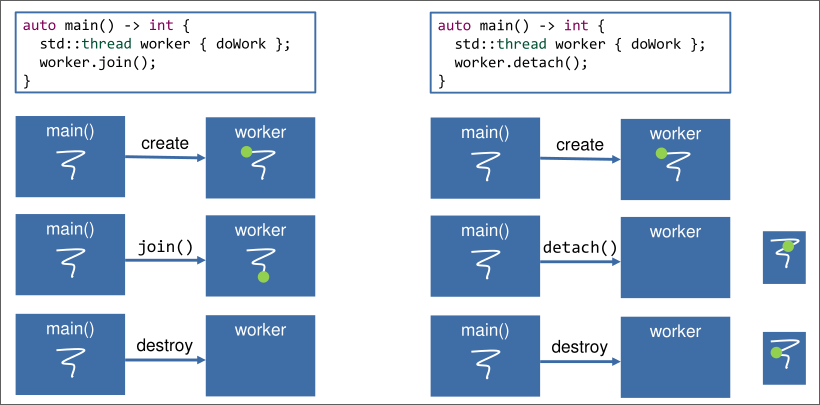
\includegraphics[scale=0.4]{2023_04_25_01_21_21.png}\newline
\textcolor{red}{Note, without .join() or .detach() your program is killed in order to avoid undefined behavior(for once).}

\subsubsection{Dangers}
\begin{lstlisting}
auto startThread() -> void {
  using namespace std::chrono_literals;
  std::string local{"local"};
  std::thread t{[&] {
    std::this_thread::sleep_for(1s);
    std::cout << local << std::endl;
  }};
  t.detach();
}
auto main() -> int {
  using namespace std::chrono_literals;
  startThread();
  std::this_thread::sleep_for(2s);
}
// problem, main thread can terminate before second thread -> therefore cout is no longer available
// cout is a global that is created with the main thread, therefore it is now a dangling reference!
\end{lstlisting}

\begin{itemize}
\item \textcolor{black}{detach or join can't be called inside destructors! -> exception problems}
\item \textcolor{black}{unjoined and undetached threads can be destroyed with \emph{std::terminate()}}
\item \textcolor{black}{when using .detach(), make sure you no longer use references from that thread -> danling references, nullptr... FUN}
\end{itemize} 

\subsection{std::jthread}
\textcolor{teal}{Thread that will automatically call .join().}
\begin{lstlisting}
auto main() -> int {
  std::jthread t {[]{
    std::cout << "Hello Thread"<< std::endl;
  }};
  std::cout << "Hello Main" << std::endl;
}
\end{lstlisting}
This thread can also be stopped by other threads with \emph{thread.request\_stop()}
\begin{lstlisting}
auto main() -> int {
  // stop token makes it possible to check how many times stop was requested
  // e.g. thread safe, and you can define how many times this will work
  // request stop is blocking
  // stop token only works with jthread
  std::jthread t {[](std::stop_token token){
    // check if stop was requested
    while (!token.stop_requested()) {
      std::this_thread::sleep_for(100ms);
    }
    std::cout << "Stop requested"<< std::endl;
  }};
  std::this_thread::sleep_for(2s);
  // request stop
  t.request_stop();
}
\end{lstlisting}

\subsubsection{iostream and threads}
IOstream is done via buffers, this is \emph{not threadsafe}, however it also does not create data races.\newline
\textcolor{teal}{What happens is that the output or input sequence is not deterministic:}\newline
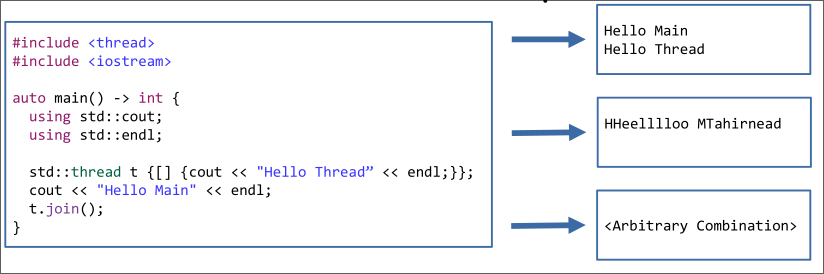
\includegraphics[scale=0.4]{2023_04_25_01_36_40.png}

\subsection{Current Thread}
There is a helper namespace \emph{std::this\_thread} which holds helper functions for the current thread:
\begin{lstlisting}
auto main() -> int {
  using std::cout;
  using std::endl;
  using namespace std::chrono_literals;
  std::thread t { [] {
    std::this_thread::yield();
    cout << "Hello ID: "
         << std::this_thread::get_id()
         << endl;
    std::this_thread::sleep_for(10ms);
  }};
  cout << "main() ID: "
       << std::this_thread::get_id()
       << endl;
  cout << "t.get_id(): "
       << t.get_id()
       << endl;
  t.join();
}
\end{lstlisting}
\begin{itemize}
\item \textcolor{purple}{get\_id()}\newline
  returns ID of current thread by the OS\newline
  This ID is unique
\item \textcolor{purple}{sleep\_for(time)}\newline
  suspends the thread for a duration
\item \textcolor{purple}{sleep\_until(time\_point)}\newline
  sleep until a certain time point
\item \textcolor{purple}{yield()}\newline
  Allows OS to schedule other threads
\end{itemize} 

\subsection{Mutexes}
\begin{itemize}
\item \textcolor{purple}{lock():} blocking
\item \textcolor{purple}{try\_lock():} non-blocking
\item \textcolor{purple}{unlock():} non-blocking
\item \textcolor{purple}{try\_lock\_for(duration):} non-blocking\newline
  try to lock for a specific duration
\item \textcolor{purple}{try\_lock\_until(time):} non-blocking\newline
  try to lock until specific time
\end{itemize} 
Mutex versions: 
\begin{itemize}
\item \textcolor{purple}{std::mutex}\newline
  standard mutex, not recursive, not timed 
\item \textcolor{purple}{std::recursive\_mutex}\newline
  recursive mutex -> allows multiple nested acquire operations of the same thread\newline
  not timed
\item \textcolor{purple}{std::timed\_mutex}\newline
  timed, not recursive -> allows try\_lock\_for() etc.
\item \textcolor{purple}{std::recursive\_timed\_mutex}\newline
  timed and recursive
\end{itemize} 
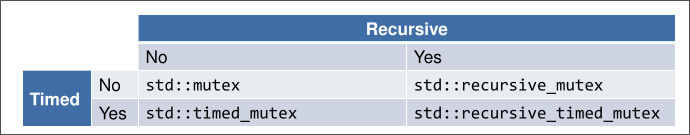
\includegraphics[scale=0.4]{2023_04_25_01_49_33.png}

\subsubsection{Read Locks}
As already covered extensively with rust, multiple reads are allowed, but not multiple writes.\newline
Hence c++ std::thread also provides read shared locks: 
\begin{itemize}
  \item \textcolor{black}{lock\_shared()}
\item \textcolor{black}{try\_lock\_shared()}
\item \textcolor{black}{try\_lock\_shared\_for(duration)}
\item \textcolor{black}{try\_lock\_shared\_until(time)}
\item unlock\_shared()
\end{itemize} 

\subsubsection{Mutex helper functions}
\begin{itemize}
\item \textcolor{black}{std::lock\_guard}\newline
  for \emph{single} mutex\newline
  locks when constructed\newline
  unlocks when destructed
\item \textcolor{black}{std::scoped\_lock}\newline
    for \emph{multiple} mutex\newline
  locks when constructed\newline
  unlocks when destructed
\item \textcolor{black}{std::unique\_lock}\newline
  defered timed locking\newline
  allows explicit locking and unlocking\newline
  unlocks when destructed (in case still locked)
\item \textcolor{black}{std::shared\_lock}\newline
  wrapper for shared mutexes\newline
  allows explicit locking and unlocking\newline
  unlocks when destructed (in case still locked)
\end{itemize} 

\subsubsection{Example for thread save queue}
\begin{lstlisting}
template <typename T,
typename MUTEX = std::mutex>
struct threadsafe_queue {
  using guard = std::lock_guard<MUTEX>;
  auto push(T const &t) -> void {
    guard lk{mx};
    q.push(t);
  }
  T pop() { /* later */ return T{};}
  auto try_pop(T & t) -> bool {
    guard lk{mx};
    // note the use of q instead of this
    // function from queue used!
    if (q.empty()) return false;
    t = q.front();
    q.pop();
    return true;
  }
  auto empty() const -> bool{
    guard lk{mx};
    return q.empty();
  }
  private:
  // mutable needed in the empty function
  mutable MUTEX mx{};
  std::queue<T> q{};
};
\end{lstlisting}
\begin{itemize}
\item \textcolor{black}{Makes every member function mutually exclusive}
\item \textcolor{black}{delegates functionality to std::queue}
\item \textcolor{black}{scoped lock pattern}\newline
  automatically locks and unlocks
\item \textcolor{black}{strategized locking pattern}\newline
  template parameter for mutex type\newline
  could also be null\_mutex(boost)
\end{itemize} 

\subsubsection{Multiple Locks with std::scoped\_lock}
\begin{lstlisting}
// can't be noexcept, because locks might throw
auto swap(threadsafe_queue<T> & other) -> void {
if (this == &other) return;

std::scoped_lock both{mx, other.mx};

argumentsstd::swap(q, other.q);
// no need to swap mutex or condition variable
}
\end{lstlisting}
\begin{itemize}
\item \textcolor{black}{acquires multiple locks in the constructor}
\item \textcolor{black}{avoids deadlocks by relying on internal sequence}
\item \textcolor{black}{blocks until all locks could be acquired}
\item \textcolor{black}{Class template argument deduction avoids the need for specifying the template arguments}
\end{itemize} 

\subsubsection{Multiple Locks without std::scoped\_lock}
\begin{lstlisting}
// can't be noexcept, because locks might throw
auto swap(threadsafe_queue<T> & other) -> void {
if (this == &other) return;

// std::defer_lock prevents immediate locking
lock my_lock{mx, std::defer_lock};
lock other_lock{other.mx, std::defer_lock};

// blocks until all locks are acquired
std::lock(my_lock, other_lock);

std::swap(q, other.q);
// no need to swap mutex or condition variable
}
\end{lstlisting}
\begin{itemize}
\item \textcolor{black}{acquires multiple locks in a single cell}
\item \textcolor{black}{avoids deadlocks}
\item \textcolor{black}{blocks untl all locks could be acquired}
\item \textcolor{black}{can also be done with try\_lock -> in that case no blocking}
\end{itemize} 

\subsection{std::condition\_variable}
\begin{itemize}
\item \textcolor{black}{Waiting for the condition}
  \begin{itemize}
  \item \textcolor{black}{wait(mutex)requires surrounding loop}
  \item \textcolor{black}{wait(mutex, predicate) loops internally}
  \item \textcolor{black}{timed: wait\_for and wait\_until}
  \end{itemize} 
\item \textcolor{black}{notifying a (potential) change}
  \begin{itemize}
  \item \textcolor{black}{notify\_one}
  \item \textcolor{black}{notify\_all}
  \end{itemize} 
\item \textcolor{black}{std::unique\_lock as condition -> releases lock}
\end{itemize} 
\begin{lstlisting}
template <typename T,
typename MUTEX = std::mutex>
struct threadsafe_queue {
  using guard = std::lock_guard<MUTEX>;
  using lock = std::unique_lock<MUTEX>;
  auto push(T const & t) -> void {
    guard lk{mx};
    q.push(t);
    // like jafuck -> other thread can activate
    notEmpty.notify_one();
  }
  auto pop() -> T {
    lock lk{mx};
    // wait for condition
    notEmpty.wait(lk, [this] {
      return !q.empty();
    });
    T t = q.front();
    q.pop();
    return t;
  }
  private:
    mutable MUTEX mx{};
    std::condition_variable notEmpty{};
    std::queue<T> q{};
};
\end{lstlisting}

\subsection{Containers}
All current standard containers are \emph{NOT thread safe}, this means that we will have to build thread safe versions of it.\newline
Note that accessing a singular element from a container is not a data race -> as singular elements are different from each other.\newline
\textcolor{teal}{Concurrent uses of containers are dangerous by default!}\newline
\textcolor{teal}{shared\_ptr copies to the same object can be used from different threads, but accessing the object
itself can race if non-const -> reference counter is atomic}

\subsection{Returns from a thread}
\subsubsection{Shared state}
We can return shared state, but this is not intuitive:
\begin{lstlisting}
auto main() -> int {
  auto mutex = std::mutex{};
  auto finished = std::condition_variable{};
  auto shared = 0;
  auto thread = std::thread{[&]{
    std::this_thread::sleep_for(2s);
    auto guard = std::lock_guard{mutex};
    shared = 42;
    finished.notify_all();
  }};
  std::this_thread::sleep_for(1s);
  auto lock = std::unique_lock{mutex};
  finished.wait(lock);
  std::cout << "The answer is:"
            << shared << '\n';
  thread.join();
}
\end{lstlisting}

\subsubsection{std::future and std::promise}
Future represent result that maybe compute asynchronously:
\begin{itemize}
\item \textcolor{purple}{wait():} blocks until available
\item \textcolor{purple}{wait\_for(timeout):} blocks until available or timed out
\item \textcolor{purple}{wait\_until(time):} blocks until available or timepoint has been reached
\item \textcolor{purple}{get():} blocks until available and returns the result value or throws if the future contains an exception
\end{itemize} 
Promises are one origin of futures:
\begin{itemize}
\item \textcolor{black}{get\_future():} obtain a future
\item \textcolor{black}{set\_result(value):} sets the associated futures result
\item \textcolor{black}{set\_exception(err):} sets the associated exception
\end{itemize} 
Usage:
\begin{lstlisting}
auto main() -> int {
  using namespace std::chrono_literals;
  std::promise<int> promise{};
  auto result = promise.get_future();
  auto thread = std::thread { [&]{
    std::this_thread::sleep_for(2s);
    promise.set_value(42);
  }};
  std::this_thread::sleep_for(1s);
  std::cout << "The answer is: " << result.get() << '\n';
  thread.join();
}
\end{lstlisting}

\subsection{std::async}
\begin{lstlisting}
// definition:
template<typename Function, typename ...Args>
auto async(Function&& f, Args&&... args) -> std::future<...>;

// usage:
auto main() -> int {
  auto the_answer = std::async([] {
    // Calculate for 7.5 million years
    return 42;
  });
  std::cout << "The answer is: " << the_answer.get() << '\n';
}
\end{lstlisting}
\begin{itemize}
  \item \textcolor{purple}{Schedules the execution of the lambda ( \emph{CAN BE IN SAME THREAD!})}
\item \textcolor{purple}{returns an std::future that will store the result}
\item \textcolor{purple}{get() waits for the result to be available}
\end{itemize} 

\subsubsection{std::async::launch and std::async::deferred}
\textcolor{teal}{std::async::launch:} forces the async to \emph{definitely use a new thread!}\newline
\textcolor{teal}{std::async::deferred:} defers execution until the result is obtained from the std::future\newline
\textcolor{red}{By default it does either of the two, so just make sure to define it!}\newline
std::aync::launch
\begin{lstlisting}
auto main() -> int {
  // new thread guaranteed
  auto the_answer = std::async(std::launch::async, [] {
    // Calculate for 7.5 million years
    return 42;
  });
  std::cout << "The answer is: " << the_answer.get() << '\n';
}
\end{lstlisting}
std::async::deferred
\begin{lstlisting}
auto main() -> int {
  // lazy evaluation, simply returns the 42 as soon as ready, in this case instantly!!
  auto the_answer = std::async(std::launch::deferred, [] {
    // Calculate for 7.5 million years
    return 42;
  });
}
\end{lstlisting}

\includepdf[pages=-,scale=1]{../cpp/cpp-typst.pdf}

\end{document}

